% ASGARD/Loki draft (verified numbers, humanized)
\appendix
\section{Separate Classification Benchmark}
\label{app:class}

A separate image-level benchmark trained seven classifier variants over five frozen similarity-group outer folds and three seeds (105 fits; 228 unique images in 209 groups; 4{,}788 out-of-fold probability rows, one prediction per image/model/seed independently verified). The full model attains mean out-of-fold macro F1 of 0.7745$\pm$0.0237 (accuracy 0.7807, AUROC 0.8457; Table~\ref{tab:class}). Removing augmentation costs the most (F1 0.6924$\pm$0.0490), while the advantage over the narrow ResNet is uncertain under descriptive unadjusted group intervals (Fig.~\ref{fig:classpairs}). This experiment shares no headline metric with the segmentation study and is reported separately by design.

\begin{table}[h]
\centering
\caption{Classification benchmark: pooled out-of-fold metrics, mean$\pm$seed SD over three seeds (105 fits).}
\label{tab:class}
\scriptsize
\begin{tabular}{lccc}
\toprule
Variant & Macro F1 & Accuracy & AUROC \\
\midrule
Full classifier & 0.7745 $\pm$ 0.0237 & 0.7807 & 0.8457 \\
No attention & 0.7346 $\pm$ 0.0096 & 0.7412 & 0.8457 \\
No multiscale & 0.7374 $\pm$ 0.0233 & 0.7471 & 0.8265 \\
Neither module & 0.7392 $\pm$ 0.0082 & 0.7485 & 0.8268 \\
No augmentation & 0.6924 $\pm$ 0.0490 & 0.7091 & 0.7466 \\
Narrow ResNet & 0.7419 $\pm$ 0.0346 & 0.7515 & 0.8040 \\
Plain CNN & 0.7120 $\pm$ 0.0562 & 0.7193 & 0.8226 \\
\bottomrule
\end{tabular}
\end{table}

\begin{figure}[htbp]
\centering
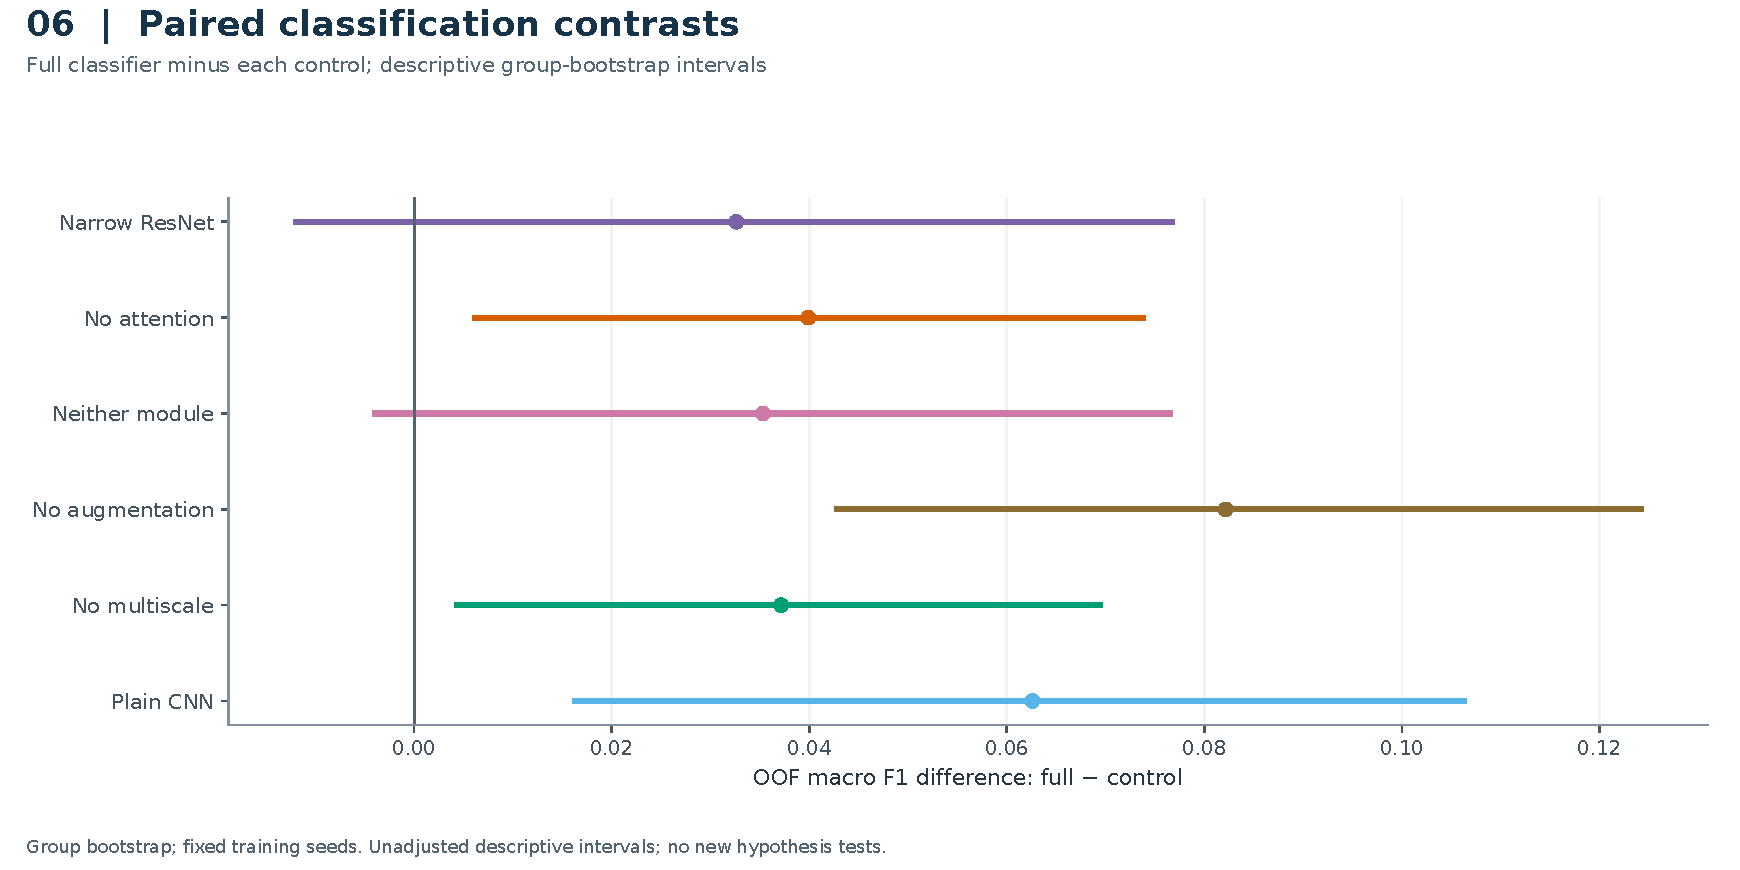
\includegraphics[width=\columnwidth]{figures/fig06_classification_paired_contrasts.pdf}
\caption{All six paired classifier contrasts with descriptive unadjusted group intervals.}
\label{fig:classpairs}
\end{figure}

